%!TEX root = ../main.tex
\section{Normed Vector Spaces}
\begin{ndfn}[Norm]
  Let $V$ be a vector space over $\R$. A norm on $V$ is a function $\norm{\cdot}:V\to\R$ with the following properties
  \begin{enumerate}
  \item $\norm{v} = 0 \iff v =0$, for $v \in V$, \hfill (definiteness)
  \item $\norm{\lambda v} = \abs{\lambda}\norm{v}$, $\forall \lambda \in \R$ and $\forall v \in V$, \hfill (absolute homogeneity)
  \item $\norm{u+v} \leq \norm{u} + \norm{v}$, $\forall u,v \in V$. \hfill (triangle inequality)
  \end{enumerate}
\end{ndfn}

\begin{ndfn}[Normed space]
  Let $V$ be a vector space, and let $\norm{\cdot}$ be a norm on $V$. The pair $(V, \norm{\cdot})$ is called a normed (vector) space.
\end{ndfn}

Some authors give a slightly different, but equivalent definition of the norm.

It should be clear from the definition that the vector space structure on $V$ is a necessity, since the axioms of being a norm rely on the existence of $0 \in V$ (the additive identity), scalar multiplication, and addition. We shall focus on the case where the underlying field is the real numbers, $\R$, however, an analogous theory can be developed in the case of other fields, for example, the complex numbers $\C$.

The idea behind defining a norm $\norm{\cdot}$ is that $\norm{x}$ should give us a measure of the \emph{magnitude} of the vector $x$. And magnitudes (or lengths) should be non-negative. So, the norms should be non-negative valued. The next result confirms this property. Some authors directly require $\norm{\cdot}:V\to[0,\infty)$, which simply gives the following proposition the status of an axiom.

\begin{nprop}[Non-negative valued]
  Let $\norm{\cdot}:V\to\R$ be a norm on $V$. Then, $\forall x \in V, \norm{x} \geq 0$.
\end{nprop}
\begin{proof}
  Observe the following
  \begin{equation*}
    0
    \overset{\text{(i)}}{=} \norm{0}
    = \norm{x+(-x)}
    \overset{\text{(iii)}}{\leq} \norm{x} + \norm{-x}
    \overset{\text{(ii)}}{=} \norm{x} + \abs{-1}\norm{x}
    = \norm{x} + \norm{x}
    = 2\norm{x}.
  \end{equation*}
  So, $2\norm{x} \geq 0$ for all $x \in V$, from which we conclude that $\norm{x} \geq 0, \forall x \in V$.
\end{proof}

Note that this proof works even when $V$ is a vector space over a general field $K$.

\begin{nprop}[Normed subspace]
  Let $(X, \norm{\cdot})$ be a normed space, and let $Y$ be a vector subspace of $X$. Then, $(Y, \norm{\cdot})$ is also a normed space, using the same norm as $X$. $(Y, \norm{\cdot})$ is called the normed subspace of $(X, \norm{\cdot})$. More precisely, this proposition claims that the function $N:Y \to \R$ with $N(y) \coloneq \norm{y}$, for all $y \in Y$, is a norm.
\end{nprop}
\begin{proof}
  Exercise.
\end{proof}

\begin{nex}
  Let $\norm{\cdot}_a$ and $\norm{\cdot}_b$ be any two norms on $V$. Do the following satisfy the definition of a norm
  \begin{enumerate}
  \item $\norm{\cdot}_a$ + $\norm{\cdot}_b$
  \item $\lambda\norm{\cdot}_a + \mu\norm{\cdot}_b$, for $\lambda, \mu \in \R$.
  \item $\norm{\cdot}_a \times \norm{\cdot}_b$
  \item $\sqrt{\norm{\cdot}_{a}}$
  \item $\norm{\left(\norm{\cdot}_b\right)}_{a}$, with the appropriate changes in domain.
  \end{enumerate}
\end{nex}

Let $V$ be a finite dimensional vector space over $\R$. Then, a result from introductory linear algebra shows that $V \cong \R^n$. Define the family of functions $\norm{\cdot}_{p}:\R^n \to \R$,
\begin{equation*}
  \norm{x}_{p} \coloneq \left(\sum_{j=1}^{n} \abs{x_j}^{p}\right)^{1/p}
  \quad\text{and}\quad
  \norm{x}_{\infty} \coloneq \max \set{x_1, \dots, x_n},
\end{equation*}
for $p \in [1,\infty)$ and $x = (x_1, \dots, x_n) \in \R^n$. Despite the suggestive notation, we have not yet claimed that these functions are valid norms.

\begin{nex}
  Show that the functions $\norm{\cdot}_{1}$ and $\norm{\cdot}_{\infty}$, are norms on $\R^n$.
\end{nex}

\begin{nex}
  Show that the function $\norm{\cdot}_{p}$, for $p \in (1,\infty)$, satisfies property (i) and (ii) of being a norm.
\end{nex}

\begin{remark}
  Indeed it will be shown later that $\norm{\cdot}_{p}$ is a norm on $\R^n$, but it will be extremely difficult to show directly that it also satisfy the triangle inequality. In order to establish the triangle inequality we will have to develop an alternative method.
\end{remark}

\begin{ndfn}
  Let $(V, \norm{\cdot})$ be a normed space. We define
  \begin{enumerate}
  \item the open unit ball: $\oB_{V} \coloneq \set{v \in V \st \norm{v} < 1}$
  \item the closed unit ball: $\cB_{V} \coloneq \set{v \in V \st \norm{v} \leq 1}$
  \end{enumerate}
\end{ndfn}
These sets depend on the norm that is being used on $V$.

The closed unit balls produced by the $\ell_{1}$, $\ell_{2}$, and $\ell_{\infty}$ norms on $\R^2$ are shown below.
\begin{center}
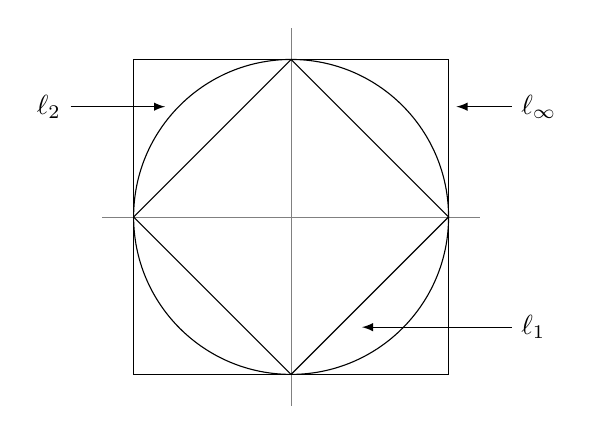
\begin{tikzpicture}[scale=2]
  \draw[help lines] (-1.2,0) -- (1.2,0);
  \draw[help lines] (0,-1.2) -- (0,1.2);
  \draw circle (1cm);
  \draw (1,0) -- (0,1) -- (-1,0) -- (0,-1) -- cycle;
  \draw (1,1) -- (-1,1) -- (-1,-1) -- (1,-1) -- cycle;

  \draw[-latex] (1.4, 0.7) node[anchor=west] {$\ell_{\infty}$} -- +(-0.35, 0);
  \draw[-latex] (-1.4, 0.7) node[anchor=east] {$\ell_{2}$} -- +(0.6, 0);
  \draw[-latex] (1.4, -0.7) node[anchor=west] {$\ell_{1}$} -- +(-0.95, 0);
\end{tikzpicture}
\end{center}

\begin{ndfn}[Convex sets]
  Let $V$ be a vector space. A set $X \subseteq V$ is called convex if $\forall x,y \in X$, and $\forall \lambda \in (0,1)$
  \begin{equation*}
    (1-\lambda) x + \lambda y \in X.
  \end{equation*}
\end{ndfn}
Geometrically, this is saying that $X$ is convex if the line segment joining any every pair of points in $X$, lies entirely within $X$.

\begin{ndfn}[Convex functions]
  A function $f : A \subseteq \R \to \R$ is called convex if $\forall x,y \in A$, and $\forall \lambda \in (0,1)$
  \begin{equation*}
    f\left((1-\lambda) x + \lambda y\right) \leq (1-\lambda) f(x) + \lambda f(y).
  \end{equation*}
\end{ndfn}
Therefore, a function is convex exactly when its graph lies beneath (or along) the line segment joining any two points on the graph. Common examples of convex functions are $x^2$ and $e^x$ on $\R$.

\begin{nprop}
  Let $(V, \norm{\cdot})$ be a normed space. The sets $\oB_{V}$ and $\cB_{V}$ are convex.
\end{nprop}
\begin{proof}
  We shall prove this for $\cB_{V}$. Take $a, b \in \cB_{V}$, and $\lambda \in (0,1)$. Then,
  \begin{equation*}
    \norm{(1-\lambda) a + \lambda b}
    \leq (1-\lambda) \norm{a} + \lambda \norm{b}
    \leq (1-\lambda) + \lambda
     = 1.
  \end{equation*}
  Therefore, $(1-\lambda) a + \lambda b \in \cB_{V}$. So, $\cB_{V}$ is convex.

  The proof for the convexity of $\oB_{V}$ is analogous.
\end{proof}

\begin{nprop}
\label{thm:convexity}
  Suppose $f \in C^2 ((a,b))$ and $f \in C^1 ([a,b])$. If $f''(x) \geq 0$, for all $x \in [a,b]$, then $f$ is convex on $[a,b]$.
\end{nprop}
\begin{proof}
  The proof is left as an exercise to the reader.
\end{proof}

\begin{nlemma}
  The function $f : \R \to [0,\infty)$ with $x \mapsto \abs{x}$ is convex.
\end{nlemma}
\begin{proof}
  To be completed. Uses the MVT.
\end{proof}

\begin{nlemma}
  The function $f : [0,\infty) \to \R$ with $x \mapsto x^p$ is convex, $\forall p \in [1,\infty)$.
\end{nlemma}
\begin{proof}
  The given function is a polynomial, so it is infinitely differentiable, with
  \begin{equation*}
    f''(x) = p(p-1)x^{p-2}.
  \end{equation*}
  Now,
  \begin{equation*}
    p \in [1,\infty), x \in [0,\infty) \implies p, (p-1), x, x^{p-2} \geq 0.
  \end{equation*}
  Therefore, $f''(x) \geq 0$, for all $x$ in the given domain.

  Proposition (\ref{thm:convexity}) then states that $f(x) = x^p$ is convex.
\end{proof}

\begin{nlemma}
  If $f: A \to B$ and $g: B \to C$ are convex functions, then $g \circ f : A \to C$ is also convex.
\end{nlemma}
\begin{proof}
  Take $x,y \in A$ and $\lambda \in (0,1)$. Then,
  \begin{align*}
  (1-\lambda) (g \circ f)(a) + \lambda (g \circ f)(b)
  &= (1-\lambda) g(f(a)) + \lambda g(f(b))\\
  &\geq g\left((1-\lambda) f(a) + \lambda f(b)\right)\\
  &\geq g\left(f\left((1-\lambda) a + \lambda b\right)\right)\\
  &= (g \circ f)\left((1-\lambda) a + \lambda b\right).
  \end{align*}
  Therefore, $(g \circ f)$ is convex.
\end{proof}

Combining these lemmas, we obtain that $\forall p \in [1,\infty)$, $x \mapsto \abs{x}^{p}$ is a convex function. In other words, $\forall x,y \in \R$, and $\forall \lambda \in (0,1)$,
\begin{equation*}
  \abs{(1-\lambda) x + \lambda y}^{p} \leq (1-\lambda) \abs{x}^{p} + \lambda \abs{y}^{p}.
\end{equation*}

Now, we consider a norm-like function that is required to satisfy all the properties except the triangle inequality. If we require the \emph{closed balls} produced by this function to be convex, then we find that it also ends up satisfying the triangle inequality. So, the next result allows us to establish the triangle inequality by checking the convexity of the induced closed balls.

\begin{nthm}
\label{thm:norm-convex-triangle}
  Let $V$ be a vector space, and consider a function $N : V \to [0,\infty)$ with
  \begin{enumerate}
  \item $N(v) = 0 \iff v =0$, for $v \in V$,
  \item $N(\lambda v) = \abs{\lambda}N(v)$, $\forall \lambda \in \R$ and $\forall v \in V$,
  \item $B \coloneq \set{v \in V \st N(v) \leq 1}$ is convex.
  \end{enumerate}
  Then,
  \begin{equation*}
    N(x+y) \leq N(x) + N(y)
  \end{equation*}
  i.e. $N$ satisfies the triangle inequality, and therefore, $f$ is a norm on $V$.
\end{nthm}
\begin{proof}
  Firstly if $N(x)=0$ then $x=0$, and
  \begin{equation*}
    N(x+y) = N(y) = N(x) + N(y).
  \end{equation*}
  Similarly, for $N(y)=0$, we have $y=0$, so
  \begin{equation*}
    N(x+y) = N(x) = N(x) + N(y).
  \end{equation*}
  Hence, assume $N(x), N(y) \geq 0$, and pick $x, y \in V$. Then, $x/N(x), y/N(y) \in V$ by closure under scalar multiplication. Moreover, $x/N(x), y/N(y) \in B$, since
  \begin{equation*}
    N\left(\frac{x}{N(x)}\right) = \abs*{\frac{1}{N(x)}}N(x) = \frac{N(x)}{N(x)} = 1.
  \end{equation*}
  Similarly for $y/N(y)$.

  By convexity of $B$ we have that
  \begin{align*}
  &\left(1 - \frac{N(y)}{N(x)+N(y)}\right)\frac{x}{N(x)} + \left(\frac{N(y)}{N(x)+N(y)}\right)\frac{y}{N(y)} \in B\\
  &\implies \left(\frac{N(x)}{N(x)+N(y)}\right)\frac{x}{N(x)} + \left(\frac{N(y)}{N(x)+N(y)}\right)\frac{y}{N(y)} \in B\\
  &\implies \frac{x+y}{N(x)+N(y)} \in B\\
  &\implies N\left(\frac{x+y}{N(x)+N(y)}\right) \leq 1\\
  &\implies \frac{N(x+y)}{N(x)+N(y)} \leq 1.
  \end{align*}
  Therefore, $N(x+y) \leq N(x) + N(y)$, as required.
\end{proof}

\begin{ncor}[Minkowski's inequality in $\R^n$]
  For all $p \in [1,\infty)$, if $x, y \in \R^n$
  \begin{equation*}
    \norm{x+y}_{p} \leq \norm{x}_{p} + \norm{y}_{p}.
  \end{equation*}
\end{ncor}
\begin{proof}
  Recall that
  \begin{equation*}
    \norm{x}_{p} \coloneq \left(\sum_{j=1}^{n} \abs{x_j}^{p}\right)^{1/p},
  \end{equation*}
  and consider the closed ball $B = \set{x \in \R^n \st \norm{x}_p \leq 1}$. Then,
  \begin{equation*}
    B = \set{x \in \R^n \st \norm{x}_p \leq 1} = \set{x \in \R^n \st \norm{x}_{p}^{p} \leq 1}.
  \end{equation*}

  We aim to show that $B$ is convex, and then use theorem (\ref{thm:norm-convex-triangle}) to obtain the triangle equality. Note that $\norm{\cdot}_{p}$ already satisfies the properties (i) and (ii) of theorem (\ref{thm:norm-convex-triangle}).

  Now, take any $x,y \in B$ and $\lambda \in (0,1)$. Then,
  \begin{align*}
  \norm{(1-\lambda) x + \lambda y}
  &= \sum_{j=1}^{n} \abs{(1-\lambda) a_j + \lambda b_j^{p}}\\
  &\leq \sum_{j=1}^{n} (1-\lambda) \abs{a_j}^{p} + \lambda \abs{b_j}^{p}\\
  &= (1-\lambda)\sum_{j=1}^{n} \abs{a_j}^{p} + \lambda \sum_{j=1}^{n} \abs{b_j}^{p} \\
  &= (1-\lambda)\norm{a}_{p}^{p}+\lambda\norm{b}_{p}^{p}\\
  &\leq (1-\lambda)+\lambda\\
  &= 1.
  \end{align*}
  Therefore, $\norm{(1-\lambda) x + \lambda y} \leq 1$; i.e. $(1-\lambda) x + \lambda y \in B$. This confirms that $B$ is convex. Theorem (\ref{thm:norm-convex-triangle}) then states that $\norm{\cdot}_{p}$ satisfies the triangle inequality. That is
  \begin{equation*}
  \norm{x+y}_{p} \leq \norm{x}_{p} + \norm{y}_{p}.\qedhere
  \end{equation*}
\end{proof}

\begin{remark}
  This completes the proof that $\norm{\cdot}_{p}$, for $p \in [1,\infty)$, as defined before, fulfils all the requirements of being a norm on $\R^n$.
\end{remark}

Next, we look at equivalent norms and the associated results for their closed (open) unit balls.

\begin{ndfn}
  Let $V$ be a vector space. A norm $\norm{\cdot}_a$ on $V$ is said to be equivalent to another norm $\norm{\cdot}_b$ on $V$ if $\exists c_1, c_2 \in \R$ with $0 < c_1 \leq c_2$, such that
  \begin{equation*}
    c_1 \norm{x}_b \leq \norm{x}_a \leq c_2 \norm{x}_b, \forall x \in V.
  \end{equation*}
  We denote this as $\norm{\cdot}_a \cong \norm{\cdot}_b$.
\end{ndfn}
It is important that the constants $c_1$ and $c_2$ are independent of the element $x \in V$. Clearly, if $\norm{\cdot}_a$ is equivalent to $\norm{\cdot}_b$, then $\norm{\cdot}_b$ is equivalent to $\norm{\cdot}_a$. In fact this is an equivalence relation. (Exercise \& Content for the appendix)

WHAT IS THE POINT OF EQUIVALENT NORMS?

\begin{nprop}
  $\norm{\cdot}_a \cong \norm{\cdot}_b$ if an only if $\exists c_1, c_2 \in \R$ with $0 < c_1 \leq c_2$, such that $c_1 \cB_b \subseteq \cB_a \subseteq c_2 \cB_b$. Here, $\cB_j$ is the closed unit ball generated by the norm $\norm{\cdot}_j$.
\end{nprop}
\begin{proof}
  The proof is left as an exercise to the reader.
\end{proof}

The previous proposition states that if $\norm{\cdot}_a$ is equivalent to $\norm{\cdot}_b$, then the closed unit ball $\cB_a$ is entirely contained within an appropriately scaled version of the closed unit ball $\cB_b$, and that $\cB_a$ also contains an appropriately scaled version of $\cB_b$. Moreover, the converse of this statement is also true.

\begin{nthm}
  All $\norm{\cdot}_p$ norms on $\R^n$ are equivalent.
\end{nthm}

In fact, a more general result holds for the case of $\R^n$: All norms on $\R^n$ are equivalent. As a result, we are free to choose any of these norm to study limits and continuity in $\R^n$, since the results will always be equivalent.

\paragraph{Some other topics of interest.} $\ell^p$ spaces, $L^p$ spaces, other norms on $\R^n$, inner products, norms on $\C^n$.